\documentclass{article}

\usepackage{fullpage}
\usepackage{amsmath, amssymb}
\usepackage{parskip}
\usepackage{bbm}

%\usepackage[backend=biber]{biblatex}
%\addbibresource{refs.bib}

\usepackage{tikz}
	\usetikzlibrary{cd,arrows,shapes}
	\usetikzlibrary{calc}
	\usetikzlibrary{decorations.pathreplacing,decorations.markings}
	\usetikzlibrary{external}
	
	\tikzset{func/.style={draw,rectangle, inner sep=1em,outer sep=0.2em}}
	\tikzset{
		% style to apply some styles to each segment of a path
		on each segment/.style={
			decorate,
			decoration={
				show path construction,
				moveto code={},
				lineto code={
					\path [#1]
					(\tikzinputsegmentfirst) -- (\tikzinputsegmentlast);
				},
				curveto code={
					\path [#1] (\tikzinputsegmentfirst)
					.. controls
					(\tikzinputsegmentsupporta) and (\tikzinputsegmentsupportb)
					..
					(\tikzinputsegmentlast);
				},
				closepath code={
					\path [#1]
					(\tikzinputsegmentfirst) -- (\tikzinputsegmentlast);
				},
			},
		},
		% style to add an arrow in the middle of a path
		mid arrow/.style={postaction={decorate,decoration={
					markings,
					mark=at position .5 with {\arrow[#1]{to}}
		}}},
	}
	\tikzset{flowc/.style={draw, postaction={on each segment={mid arrow}}}}

%\tikzexternalize[optimize=false]
%\tikzsetexternalprefix{figs/}

	
\usepackage{amsthm}

\usepackage{thmtools}
\declaretheoremstyle[%
spaceabove=-3pt,%
spacebelow=12pt,%
headfont=\normalfont\itshape,%
postheadspace=1em,%
qed=\qedsymbol%
]{mystyle} 
\declaretheorem[name={Proof},style=mystyle,unnumbered,
]{prf}

\newtheorem{lemma}{Lemma}
\newtheorem{note}{Note}
\theoremstyle{definition}
\newtheorem{claim}{Claim}
\newtheorem{defn}{Definition}


\newcommand{\Z}{\mathcal Z}

\begin{document}
	
	\section{Motivation}
	\textbf{Changes of Heart.} The standard picture of an agent is a system trying to maximize a fixed reward function, or satisfy some fixed set of preferences. However, humans usually either do not always have preferences, or have very poor access to them. Moreover, they often seem to change their fundamental goals, and form new preferences about things they had previously never experienced or understood. 
	
	The standard response to this is that really the humans must had have a deeper, higher level goal all along, and that they now have realized that this goal would be better serviced with a different instrumental goal. For rational agents with a fixed reward function do not change their preferences, except insofar as they have totally misunderstood what their actions actually do. 
	
	To be clear, this is a perfectly coherent view: humans change their preferences because they are flawed reasoners, and truly rational beings would never do such a thing. Perhaps you were giving money to your kids because you didn't realize that you could have made a bigger impact by donating it to a charity, or perhaps because there is some uncertainty about how effective the charity actually is. And then when you visit the slums of India, you realize that (despite being a kind, positive person being your goal all along). According to this view, morality is an accident, and corresponds to a very deep preference that every person is born with --- and any extent to which this picture doesn't seem right, is because you are merely a flawed mortal.
	
	However, it is not a view that feels subjectively correct; the things you care about on a deep level seem to genuinely change: it seems possible to visit a place of poverty and empathize with people to the point of changing priorities, without learning any new facts about the severity of the situation. Moreover it suffers a number of issues on the developmental front: complicated platonic ideals of meta-preferences seem unlikely to be already fully-formed in toddlers, especially given that self-awareness develops at 18 months, and even 5 year-olds stick to simplistic, causal answers to ethical questions.
	
%	Ultimately, changes of mind are well-studied and understood, but changes of heart are almost entirely dismissed as flawed behavior of humans. This is the 

	\textbf{AI Safety Concerns}. Using this framework, we have built a substantial theory of how we can use clever optimization techniques to maximize rewards, formulating reinforcement learning (RL). Supervised and unsupervised learning problems can be formulated as restrictions on the general RL problem. A great deal of the problems with learned models are due to overfitting.
	
	
	We are interested in questions:
	\begin{enumerate}
		\item Can we explain agents' changes of preference without appealing to higher ideals, or by simply stating that humans are flawed? In particular, can we use this theory to explain how values get captured by gamification (grades capturing learning, steps capturing exercise)? 
		\item The practice of 
		\item Is it evolutionarily beneficial 
		\item How does this relate to the problems 
		\item What implications does this have for designing
	\end{enumerate}
	
	
	
	, as well as the development of a more general class of reward functions, we must first develop a formal picture of agency, so that we may capture the notion of a ``sub-agent'', and understand how a reward might arise.
	
	\subsection{Motivating Examples}
	
	\section{Related Questions and Previous Work}
	\subsection{The Orthogonality Hypothesis}
	
	
	\section{Cartesian Agents}
	We will develop the discrete case first: an ascription of agency to a nondeterministic process, how it can be extended in the case that the non-determinism comes with probabilities (i.e., is a Markov Process).
	
	
	\subsection{General Non-deterministic Processes}
	
	At its very most basic, our input is a space $\Z$, of all possible states that the system could be in, plus a non-deterministic function	
	\[ \tau: \Z \to 2^{\Z} \] 
	
	which describes the allowable next states from any given current state.
	We can also draw this as a \textit{string diagram}, akin to a circuit or process diagram, in which the nodes are functions, and are connected by typed wires which are thought of as carrying data.
	
	\begin{center}
		\begin{tikzpicture}		
			\node[anchor=north, inner sep=0.6em] (A) at (0,0) {$\Z$};
			\node[func] (t) at (0,1){$\tau$};
			
			
			\draw[->] (t) -- ++(2,0) -- ++(0,-1) -- (A.north);
			\draw[<-] (t) -- ++(-2,0) -- ++(0,-1) -- (A.north);
		\end{tikzpicture}
	\end{center}
	
	This picture would make sense if the system were deterministic (and $\tau$ were a function $\Z \to \Z$), but since the output of $\tau$ is technically different from its input, we need some choice to close the loop like this --- like, for example, a function $\chi: 2^\Z \to \Z$, which selects one of the possible next states.
	
	\begin{center}
		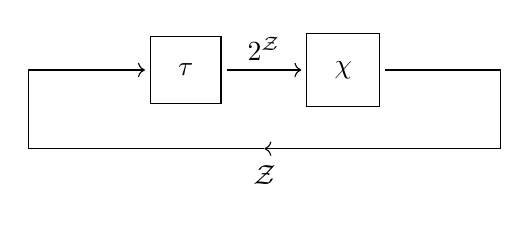
\begin{tikzpicture}		
		\node[anchor=north, inner sep=0.6em] (A) at (1,0) {$\Z$};
		\node[func] (t) at (0,1){$\tau$};
		\node[func] (c) at (2,1){$\chi$};
		
		
		\draw[->] (c) -- ++(2,0) -- ++(0,-1) -- (A.north);
		\draw[->] (t) -- node[above]{$2^\Z$} (c);
		\draw[<-] (t) -- ++(-2,0) -- ++(0,-1) -- (A.north);
		\end{tikzpicture}
	\end{center}

	This picture, too, is somewhat misleading, since there are many functions from $2^{\cal Z} \to \cal Z$ which do not always select a member of the subset in question. To add the appropriate restrictions, we require that $\chi\circ\tau$ is \textit{compatible} with $\tau$ in the following sense:
	
	\vspace{1em}
	\begin{defn}
		A function $f : \Z \to \Z$ is \emph{compatible} with a non-deterministic function $\tau : \Z \to 2^\Z$, and we write $f : \tau$, iff $\forall z \in \Z. f(z) \in \tau(z)$, or equivalently, if
		\begin{center}
			\begin{tikzcd}
				\Z \times \Z  \ar[r, "\tau \times f"] & 2^\Z \times \Z \ar[r,"\mathrm{ev}_{\Z,2}"]& 2 \\
				\Z \ar[u, "\Delta"] \ar[rr]&&* \ar[u, "\top"']
			\end{tikzcd}
		\end{center}	
		\vspace{1em}	
	\end{defn}
	
	\begin{defn}
		More generally, $f : \Z \to 2^\Z$ is \emph{compatible} with $\tau : \Z \to 2^\Z$, and we write $f \subseteq \tau$ iff $\forall z \in \Z. f(z) \subseteq \tau(z)$.
	\end{defn}



	One can see how $\chi$ can be considered an ``agent'', as it is making the relevant choices. However, this may not be the only way of ascribing agency, and may in fact be far off from what we would normally consider an agent: such an agent may be making choices about very unrelated things in a very large universe. If we interpret the laws of physics in this framework, then this agent is an all-powerful being which makes all choices at every time-step; we want a way of breaking this into smaller pieces.


	We want to also (at the very least) allow for a separation between individual choices which are independent from one another, and allow for some subset of the non-determinism to be interpreted without agency. 
	
	\subsection{System Factorization}
	\begin{defn}
		An agent factorization of $\Z, \tau : \Z \to 2^\Z$ is a tuple $(\mathcal A, X, Y, \eta, \nu)$, where
		
		\begin{itemize}\setlength\itemsep{-0.4em}
			\item $\cal A$ is a collection of agents
			\item $X = \prod_{a : \cal A} X_a$ and $Y = \prod_{a : \cal A} Y_a$ are the input and output spaces, indexed by agent
			\item $\eta: \Z \to \prod_{a: A} X_a$ is a function with components $\eta_\alpha: \Z \to X_\alpha$ for each $\alpha \in \cal A$, which constructs the input for agent $\alpha$ for a given state of the world
			\item a function $\nu: \Z \times (\prod_{\alpha: \cal A} Y_\alpha) \to 2^\Z$ which uses the previous state of the world and all of the agents' choices to specify a set of possible outcomes
		\end{itemize}
		whose composition is compatible with $\tau$, no matter what choices the agents make. More precisely, for any collection of functions $\{F_\alpha: X_\alpha \to Y_\alpha\}_{\alpha : \cal A}$, we have
		
		\begin{equation} \label{eq:same}
		\nu \circ \left[ \mathrm{id}_\Z  ~\otimes~ \left(\bigotimes_{\alpha : \cal A} F_\alpha \right) \eta \right] ~\subseteq~\tau
		\end{equation} 
	\end{defn}
	
	
	With string diagrams, we have the following picture:
	\vspace{1em}
	\begin{center}
		\begin{tikzpicture}
		\node[anchor=north, inner sep=0.6em] (A) at (0,0) {$\cal Z$};
		
		\node[func] (e) at (-2,2){$\eta$};
		\node[func] (a1) at (0,2.8){$F_\alpha$};
		\node (andsoon) at (0,2.1) {$\vdots$};
		\node[func] (a2) at (0,1.2){$F_\beta$};
		\node[func] (n) at (2,2){$\nu$};
		
		\path[flowc] 
			(e) to[out=10,in=180] (a1) (a1) to[out=0,in=170] (n)
			(e) to[out=-10,in=180] (a2) (a2) to[out=0,in=190] (n);
		
		
		\path[draw] ($(e)+(-2,0)$) -- ++(0,2) edge[mid arrow] ($(n)+(0,2)$) ($(n)+(0,2)$) edge[->] (n);
		\draw[->] (n) -- ++(2,0) -- ++(0,-2) -- (0,0);
 		\draw[<-] (e) -- ++(-2,0) -- ++(0,-2) -- (0,0);
		
		\end{tikzpicture}
	\end{center}

	If, more than simply being compatible with $\tau$, the subset relation in equation \eqref{eq:same} is replaced with set equality, then we have exactly captured the nondeterminacy of the system by the choices we expose via the types $X_\alpha$ and $Y_\alpha$. More formally,
	
	\vspace{1em}
	\begin{defn}
		We will call an agency factorization $(\mathcal A, X, Y, \eta, \nu)$ of $(\tau, \cal Z)$ \emph{complete} if
		\begin{equation*} 
		\nu \circ \left[ \mathrm{id}_\Z  ~\otimes~ \left(\bigotimes_{\alpha : \cal A} F_\alpha \right) \eta \right] ~=~\tau
		\end{equation*} 
		%$\langle F_\alpha \rangle$
	\end{defn}

	\vspace{1em}
	\begin{note}
		An agent factorization is complete if and only if, for any $z \in \Z$ and $z' \in \tau(z)$, there exists some collection $\{F_\alpha\}$ such that $z' \in \nu(z, \{F_\alpha\eta_\alpha(z)\})$.
	\end{note}


	Of course, there's always the trivial factorization, with no agents, trivial $\eta$, each $X_\alpha = Y_\alpha = *$, and $\nu = \tau$, corresponding to the view that everything is deterministic and there are no real choices worth ascribing agency to. 
	
	
	However, we want to focus on factorizations that make sense in terms of agency or influence.
	Below we go through some different ways this might be done.

%	\subsection{Counterfactuals}
%	 we want it to be the case that I \emph{could} have chosen something different --- which is to say, by intervening only on the part of the world which specifies the code for $\alpha$, one could have caused a different decision.
%	 
%	 
%%	I want to capture the fact that agents have choices: that is, it is possible that they could have done something differently (i.e., if their algorithms worked slightly differently). 
%	
%	More precisely, we want any function $\alpha' : X_\alpha \to Y_\alpha$, of the same domain and co-domain as $\alpha$ (thought of as an alternate decision you could have made), to be somehow consistent with $\tau$, given that you change the bits of $Z$ which encode properties of $\alpha$. Therefore, we also need a function $\epsilon: \mathcal A \to \mathcal P(Z)$ denoting the subset of $\cal Z$ which encodes the functionality of $A$. 
%	
%	For every $\alpha' : X_\alpha \to Y_\alpha$,
%	\begin{enumerate}
%		\item $\epsilon \alpha = \epsilon \alpha'$ (the category is flat)
%		\item There is some $\delta_{\alpha}^{\alpha'} : \epsilon \alpha \to \epsilon \alpha$, such that \[\tau \circ (\delta_\alpha^{\alpha'} \otimes \mathrm{id}_{Z \backslash \epsilon \alpha})
%		\]
%	\end{enumerate}
%	
%	\[ \nu \circ \left[ \left(\bigotimes_{\alpha : \cal A} \alpha' \right) \eta ~\otimes~ \mathrm{id}_{\cal Z} \right] (z) \subseteq \tau(z) \]
%	
%%	\[ \nu \alpha'\eta\delta_\alpha^{\alpha'} = \tau \delta_\alpha^{\alpha'} \]
%	
%	
%	\subsection{Additional Conditions}
%	There are many factorizations of this form that tell us nothing. To cut down on these, we will impose some additional restrictions and metrics for evaluating the quality of such a factorization.
%	
%	\textbf{Choices}. Each $Y_\alpha$ needs to be non-terminal.
%	
%	\textbf{Meaningful Choices.} $\nu$ depends on the inputs $\alpha : \cal A$.
%	
%	
%	
%	
%
%	\subsection{Code}
%	Alternatively, we want a decomposition of $\cal Z$ into algorithms, and data.
%	
%	\section{Sub-agents}
%	
%	$ A \leqslant B$ if there exists a function $f: $
%	
%	
	\section{Evolution}
	
	
	\subsection{The Red Queen}
	
	\section{Formalism}
	%	In the simple case, we require the following data: 
	
	\begin{tabular}{r|l}
		$\cal Z$ & Space of information in the world \\
		$\tau: {\cal Z \to Z} \to \Omega$ & Evolution of the world agents in it \\
	\end{tabular}
	\vspace{1em}
	
	
	\begin{tabular}{r|c|l}		
		$\cal A : U$ && Set of agents \\[0.3em]
		$\displaystyle X: \prod_{\alpha: A} X_\alpha$ & $X_\alpha$ & Input type for agent $\alpha$ \\[1.7em]
		$\displaystyle Y: \prod_{\alpha: A} Y_\alpha$ &$Y_\alpha$ & Set of actions for agent $\alpha$ \\
		$\displaystyle \epsilon: \mathcal A \times \Z \to \Omega $&$\epsilon_\alpha \subseteq \cal Z$ & Subspace of $Z$ that determines behaviors of $\alpha$ \\
		$Q_\alpha: \epsilon\alpha \to X_\alpha \to Y_\alpha$ & x 
	\end{tabular}
	
\end{document}